\documentclass{../industrial-development}
\graphicspath{{14-leadership-and-development-team-management/}}

\title{Лидерство руководителя и управление командой разработчиков}
\author{Грязева А.И. Камуз А.В. ИВТ-21 МО}
\date{}

\begin{document}

\begin{frame}
  \titlepage
\end{frame}

\section{Кто такой руководитель}


\begin{frame} \frametitle{Понятие руководителя}

\begin{block}{Определение:}
Руководитель команды разработчиков--- это IT-специалист, который \alert{управляет командой} разработчиков, владеет технической стороной, принимает участие в работе над~архитектурой проекта, занимается ревью кода, а также разработкой некоторых особо сложных заданий на проекте
\end{block}
\end{frame}
\lecturenotes Руководитель команды разработчиков как профессия возникла относительно недавно. Когда компьютерные технологии начали активно развиваться, стало понятно, что для работы над IT-проектами требуется целый коллектив сотрудников. Для организации их деятельности понадобился человек, который не только разбирается в создании веб-продукта, но и способен скоординировать и оптимизировать работу группы. На сегодняшний день руководитель команды разработчиков – это важнейшее звено между заказчиком и разработчиками.
Он распределяет задания между участниками группы, планирует релизы и их выпуск, отвечает за дизайн, разработку и маркетинг, следит за профессиональным ростом сотрудников, проводит совещания, отчитывается о проделанной работе перед заказчиком. 
В обязанности руководителя входит составить техзадание на основе бизнес-задачи, написать ревью-код, решить возникшие проблемы, оптимизировать работу, выгрузить продукт на боевой сервер. Он участвует в разработке и тестировании проекта, контролирует его качество и технологию исполнения.





\begin{frame} \frametitle{Качества руководителя}

  \begin{itemize}
  \item Ответственность: для того чтобы не бояться принимать решения и нести личную ответственность за решения 
  \item Дипломатичность: для того чтобы успешно разрешать возникающие конфликты и противоречия. Без этого качества не обойтись в ситуации, когда руководителю необходимо указать разработчику на недостатки в его работе
  \item Самосовершенствование: руководитель должен замечать и исправлять слабые места в своем руководстве
  \item Оптимизм: руководителю необходимо воодушевлять разработчиков на достижение целей
    \end{itemize}
  \end{frame}

   
\begin{frame} \frametitle{Качества руководителя}

  \begin{itemize}
  
  \item Уверенность: уверенный руководитель должен быть уравновешен и спокоен. Это положительно влияет на~атмосферу работы разработчиков 
 \item Стрессоустойчивость: удерживание команды от~излишних эмоций, умение быстро принимать ответственные решения при разных обстоятельствах
 \item Коммуникабельность: способность построить систему коммуникаций в команде, получать надежную информацию и эффективно ее оценивать
 \item Лидерство: руководитель должен уметь вести за собой сотрудников, мотивировать их на достижение целей
  \end{itemize}
\end{frame}

\lecturenotes Руководитель - это трудолюбивый, ответственный человек с аналитическим складом ума. Он пунктуален, дипломатичен, инициативен, умеет находить общий язык с разными людьми, организовать работу команды и сплотить коллектив. Также руководитель способен быстро принимать решения, работать в стрессовом режиме, выбирать наиболее простые и действенные методы разрешения проблемы, для него на первом месте стоит результат работы. Руководитель готов учиться, он умеет смотреть на проблему с разных точек зрения и прислушиваться к мнению коллег



\section{Кто такой лидер}

\begin{frame} \frametitle {Понятие лидера и лидерства}

\begin{block}{Определение:}
Лидерство --- \alert{способность влиять} как на отдельную личность, так и на группу, направляя усилия всех на~достижение целей компании
\end{block}
Это социально-психологический процесс, основанный на влиянии личного авторитета человека на~поведенческий аспект группы



\begin{block}{Определение:}
Лидер --- это человек, который может \alert{влиять} на поведение других людей, \alert{брать} на себя \alert{ответственность}, последовательно \alert{идти к достижению} конкретных \alert{целей} и~\alert{вести} за собой \alert{команду}
\end{block}

\end{frame}

\lecturenotes Под влиянием понимают такое поведение человека, которое приводит к изменениям в действиях, отношениях, чувствах другого человека. Влияние можно оказывать через идеи, устное и письменное слово, внушение, убеждение, эмоциональное заражение, принуждение, личный авторитет и пример.
Неотъемлемый атрибут лидерства — наличие хотя бы одного последователя. Важно умение повести людей за собой, обеспечить существование таких системных связей между ними, которые бы способствовали решению конкретных задач по достижению единой цели.
Лидерство — всегда вопрос степени, силы влияния, зависящей от соотношения личных качеств авторитетной личности с качествами тех, на кого она пытается оказать влияние, и. с ситуацией, в которой находится данная группа

\begin{frame} \frametitle{Виды лидерства}
Характеристика стилей лидерства по преобладающим функциям определяет такие виды: 
  \begin{itemize}
  \item Лидер-организатор 
  \item Лидер-творец
  \item Лидер-борец  
  \item Лидер-дипломат
  \item Лидер-утешитель
  \end{itemize}
\end{frame}

\begin{frame} \frametitle{Лидер-организатор}

\begin{itemize}
  \item Воспринимает нужды коллектива как собственные 
  \item Умеет убеждать
  \item Уверен, что большинство проблем разрешимы, оптимистичен
  \item Склонен поощрять, выражает неоодобрение не задевая достоинства коллеги
  \end{itemize}

\begin{block}{Результат:}
Конструктивная критика способствует возникновению желания работать лучше у членов команды. Если~лидер-организатор ставит задачу, то она будет четкой и~выполнимой
\end{block}
\end{frame}
\lecturenotes Лидер-организатор – это вид лидера, который считает желания группы своими собственными. Такой тип лидера склонен к активным действиям, он уверен в себе и оптимистичен. За лидером-организатором следуют, зная, что он не будет предлагать не действенные варианты. Он может убедить, поощрить. В случаях, когда лидер недоволен каким-либо членом группы, негодование свое он высказывает, не задевая чужого достоинства. А это, в свою очередь, мотивирует людей на лучшую работу



\begin{frame} \frametitle{Лидер-творец}
\begin{itemize}
  \item Способен видеть перспективу и внедрять новое
  \item Отсутствует необходимость командовать коллегами --- следование по собственному желанию
  \item Умеет заинтересовать команду решением задачи или~возникшей проблемы 
  \end{itemize}
  \begin{block}{Результат:}
	Наличие оригинальных идей приводит к сплоченности коллектива вокруг лидера-творца. Он вдохновляет команду на решение сложных задач
  \end{block}
\end{frame}
\lecturenotes Лидер-творец способен видеть и внедрять новое и неизвестное, что притягивает коллег. У лидера-творца не возникает необходимости командовать людьми – они следуют за ним по собственному желанию. Особенностью такого стиля лидерства можно назвать то, что, приглашая к обсуждению, такой лидер умеет сформулировать возникшую проблему или задачу таким образом, что члены коллектива заинтересуются ее решением и начнут действовать по доброй воле.



\begin{frame} \frametitle{Лидер-борец}
\begin{itemize}
  \item Уверен в своих силах, бескомпромиссен
  \item Готов отстаивать свои убеждения и мнения коллектива 
  \item Является сильным, волевым лидером
  \end{itemize}
\begin{block}{Результат:}
Лидер-борец не всегда в состоянии предусмотреть последствия своих действий, в борьбе может забывать о~рациональности и лояльности, что может навредить общим интересам команды
\end{block}
\end{frame}
\lecturenotes Лидеру-борцу свойственны воля и уверенность в своих силах. Он не уходит от опасности и всегда готов к атаке, отстаивая свои убеждения и мнения коллектива, он довольно бескомпромиссный. Конечно, в таком стиле лидерства можно наблюдать недостатки: лидер не всегда в состоянии предусмотреть последствия своих действий.

\begin{frame} \frametitle{Лидер-дипломат}
\begin{itemize}
  \item Не афиширует о своих планах
  \item Умеет манипулировать людьми незаметно для них самих
  \item Отдает предпочтение доверительным встречам с~членами команды
  \item Готов выслушать собеседника
  \end{itemize}
  \begin{block}{Результат:}
   Лидер-дипломат опирается на отличное знание ситуации и~ее невидимых деталей. Хорошо управляет командой, так~как всегда в курсе всех отношений в коллективе и~осведомлен в том, как и на кого можно повлиять	
  \end{block}
\end{frame}
\lecturenotes Лидер-дипломат хорошо владеет ситуацией, находится в курсе событий, которые происходят в команде, знает на кого и как можно влиять. Отдает предпочтение доверительным встречам в кругу единомышленников. Старается менять тему разговора, чтобы увести внимание собеседников от своих планов. Такой стиль лидерства в организации всегда делает ставку не на прямолинейность и открытость, а на скрытые и замаскированные способы воздействия.


\begin{frame} \frametitle{Лидер-утешитель}
\begin{itemize}
  \item Готов поддержать в трудную минуту
  \item Обладает вежливостью, предупредительностью и~сопереживанием
  \item Прислушивается к мнению коллектива в целом и~к~каждому его члену в отдельности
  \item Отличается почтительностью и благожелательностью
  \end{itemize}
  \begin{block}{Результат:}
Лидеру-утешителю может не доставать объективности и~организованности, без которых невозможно успешно вести команду, однако к нему в коллективе всегда будут расположены доброжелательно
  \end{block}
\end{frame}
\lecturenotes Лидер-утешител наделен превосходными человеческими качествами. Он склонен сопереживать, поддержать человека в трудную минуту. Всегда вежлив и предупредителен, может выслушать человека и вникнуть в его проблемы, к нему в коллективе всегда будут расположены доброжелательно.



\begin{frame} \frametitle {Основные принципы лидерства для руководителя}

\begin{itemize}
	\item Понимание: определитесь с тем, куда вы идете
	\item Передача знаний: делитесь своими знаниями так, чтобы подчиненные все поняли
	\item Делегирование: общие задачи нужно решать общими усилиями
	\item Проверка: проверяйте свои действия и то, что делают ваши подчиненные в контексте достижения 	поставленных целей
	\item Участие: погружайтесь в работу с головой --- будьте примером для остальных
\end{itemize}
\end{frame}
\lecturenotes Понимание
Прежде чем приступать к обязанностям, лидер должен определить, в каком направлении он поведет своих подчиненных. Он должны полностью понять для себя цели компании – лишь в этом случае можно донести их до подчиненных. Процесс изучения начинается с перспективного представления. Лидер программистов не может себе позволить заблудиться – слишком серьезными могут быть последствия и для подчиненных, и для продукта. Для комплексного понимания проблемы необходимо обдумать и обосновать каждое коммерческое требование. Наивно надеяться на то, что сотрудники, прочитав спецификацию продукта, все сразу поймут и создадут реализацию именно такой, как требуется. Только выстроив подробный план реализации от начала до конца, лидер сможет руководить процессом и отслеживать его. Здесь необходимы время и настойчивость. План анализа проблемы можно изложить следующим образом. 
1. Прочтите требования дважды: один раз, чтобы понять широту замысла, второй – чтобы постичь его глубину.
2. Сопоставьте требования с известными методиками реализации и выявите те части функциональности, для реализации которых потребуются новые разработки. 
3. Набросайте предварительный план макетирования проектов – он поможет выявить среди требуемых свойств неизвестные. 
4. Составьте на основе документации с требованиями контрольный список, который, в свою очередь, послужит исходной точкой для формулирования задач. Так вы сможете привязать каждое требование к набору задач и тем самым гарантировать реализацию свойства. Понимание рождает решения.


\lecturenotes Передача знаний

Способность передавать знания есть второй необходимый признак лидера. Недостаточное понимание проблемы порождает комплекс, в результате чего субъект, который, по смыслу, должен эту проблему доходчиво изложить, начинает надеяться на то, что окружающие смогут интуитивно разобраться в ней и уяснить свои задачи.
Цель передачи знаний – обеспечить понимание персоналом предъявленных к продукту требований на том же уровне, на котором их понимает лидер. 
Тот, кто способен четко доносить свои знания до окружающих, сможет преуспеть в педагогике.
Многие лидеры излишне увлекаются стилем – в основном по той причине, что у них не все в порядке с содержанием. Основное внимание нужно уделять содержанию, а тонкости изложения можно будет наработать с опытом. Необходимо различать запланированный процесс передачи знаний и случайные разговоры на ту или иную тему. Большую часть жизни мы доносим до окружающих информацию интуитивно, не пользуясь заготовками и отталкиваясь исключительно от текущего контекста. Различия между бессистемным и формальным мышлением следует обязательно иметь в виду; бывают ситуации, когда случайно высказанная мысль приводит к непредусмотренным разрушительным последствиям для бизнеса.
Как лучше всего донести до программиста суть требований? Показать ему частично функционирующий макет. Даже одни пользовательские интерфейсы способны помочь программисту составить представление о задаче. Но не стоит сбрасывать со счетов архитектуру. Впрочем, строить разработку программных средств исключительно на основе документов не стоит. Нередко такие важные элементы процесса передачи знаний, как макетирование и критический обзор предварительных аспектов реализации, просто-напросто игнорируются. Конструирование макетов как средств передачи знаний приносит пользу в двух отношениях: во-первых, удовлетворяет привычку к кодированию, вовторых, помогает донести до окружающих ваше понимание решения поставленной задачи.


\lecturenotes Делегирование
Объяснив подчиненным, какая задача перед ними стоит, необходимо заставить их ее решить. Способность к делегированию – это одно из тех качеств, которое лидер должен постоянно совершенствовать. 
В идеале проект нужно разбить на рабочие единицы, которые впоследствии можно будет распределить между всеми разработчиками. для решения отдельных задач по проекту или даже для комплексной его реализации лучше всего подходит ограниченная группа сотрудников. Иногда, программистов имеет смысл разбивать по парам. В рамках этой методики также культивируется другой тип делегирования – он предусматривает создание команды из двух программистов, в которой один пишет код, а другой ежедневно тестирует его и проводит критические обзоры. Если подобрать подходящих кандидатов (лучше всего – опытного программиста и новичка), эта схема делегирования оказывается очень эффективной. Однако если подобрать партнеров неверно, присущая программистам независимость сведет эффективность этой замечательной идеи нулю. Помимо прочих навыков делегирования, лидер должен понимать, какие из сотрудников могут работать вместе, а какие – нет.
Делегировать можно задачи, но не темпы их решения. Если разбить проект на отдельные задания трудно, значит, возможно, проблема кроется в проектном решении и плану конструирования недостает модульности. Иногда в самом начале работы над проектом кажется, что никаких проблем с делегированием не возникнет. Но впоследствии, выясняется, что одни группы уже решили поставленные перед ними задачи, а другие запаздывают. Подобные ситуации возникают из-за неверного представления о продолжительности выполнения тех или иных заданий. Качественное проектное обеспечивает удобство делегирования по модулям.

\lecturenotes Проверка 
Естественная задача, возникающая после делегирования, заключается в контроле за ходом выполнения заданий. Лучший способ приблизить перспективу завершения проекта в срок – проводить регулярные сборки компонентов вплоть до полной готовности кода. Такие действия, помимо прочего, помогают избежать попадания в проектный тупик. Слишком много времени теряется, если на подходе к завершению цикла разработки приходится начинать все сначала – по той лишь причине, что проектное решение себя не оправдало. Одним из элементов вашей повседневной деятельности должна стать ежедневная проверка результатов работы сотрудников; при приближении сроков сдачи такие проверки нужно проводить еще чаще. 
Некоторые методики проверки: 
1)Лидер ежедневно должен интересоваться как обстоят дела у подчиненных. Если личный контакт не представляется возможным необходимо связаться с коллегами 
2)С регулярностью в несколько дней лидер должен тестировать готовые модули кода. Данную деятельность он должен воспринимать, как свою первоочередную. 
3)Лидеру необходимо интегрировать компоненты в целостную систему и проверять архитектуру на стройность. Так он сможет выявлять ошибки, допущенные при конструировании, и держаться в курсе методов, которыми программисты решают поставленные перед ними задачи. 
4)Проводя еженедельные совещания сотрудников, лидер должен отслеживать состояние проекта и вырабатывать вместе с подчиненными новые идеи. Эта деятельность дополняет ежедневные визиты к сотрудникам и позволяет привлечь к решению проблем общего характера коллективный разум. 
5)Тех участников группы разработчиков, которым удалось быстро расправиться со своими задачами, следует привлекать к тестированию результатов. Программирование не ограничивается написанием кода, оно также предполагает обеспечение его реального функционирования. 
8)Лидер должен требовать от программистов документировать все новые модули кода и составлять из этих отчетов сопроводительную документацию для отдела тестирования. Тем самым вы дадите возможность себе и своим подчиненным оценивать ход процесса и соответствие заданным требованиям. 
Вышеупомянутые методики помогают превратить процесс мониторинга в продуктивную и конструктивную деятельность, не ограничивающуюся критикой. Если лидер не будет проверять своих подчиненных, кто-нибудь из них может выпасть из общего темпа разработки, вследствие чего продукт не будет сдан вовремя. Достичь сопоставимых успехов в разработке должны все участники группы – в противном случае толку от такой деятельности будет очень мало



\lecturenotes Участие
 Лидеру нередко придется участвовать в процессе кодирования. Если сочетать эту деятельность с делегированием и проверкой, ничего страшного не произойдет. Участие написании кода поможет утвердиться в роли лидера, хотя здесь нужно стараться воздерживаться от мелочной опеки. С учетом численности персонала отдела эта деятельность может стать необходимостью, однако за написание кода, с одной стороны, и организацию этого процесса, с другой, отвечают разные участки мозга. Переключаться с одного вида деятельности на другой довольно сложно. Для ведения административных дел далеко не всегда требуется такая же концентрация, как для программирования; таким образом, исполняя обязанности руководителя, можно позволить себе отвлечься на телефонный звонок или письмо, пришедшее по электронной почте.
В работе руководителя необходима концентрация – любой специалист в области разработки программных средств должен стремиться в каждый конкретный момент заниматься чем-то одним.

Участие руководителя в кодировании зачастую сводится к тестированию. Это жизненный пример участия лидера в процессе. Готовьтесь к нетривиальным испытаниям ваших технических навыков и учитесь рационально использовать время. Справившись с этими трудностями, руководитель сможет укрепиться в положении лидера. Разработка программных продуктов – это не спринт, а марафон; в этом контексте умение взять правильный темп есть необходимое условие стабильной работы всей команды. Чтобы выиграть марафон, нужно поддерживать взятый темп, прилагать усилия к тому, чтобы переставлять ноги, следить за рельефом и не забывать, как это здорово – пересечь финишную линию с достойным временем.
Участие – это способность пробежать всю дистанцию, ни разу не теряя внимания.


\begin{frame} \frametitle{Основные принципы лидерства}
\begin{center}
  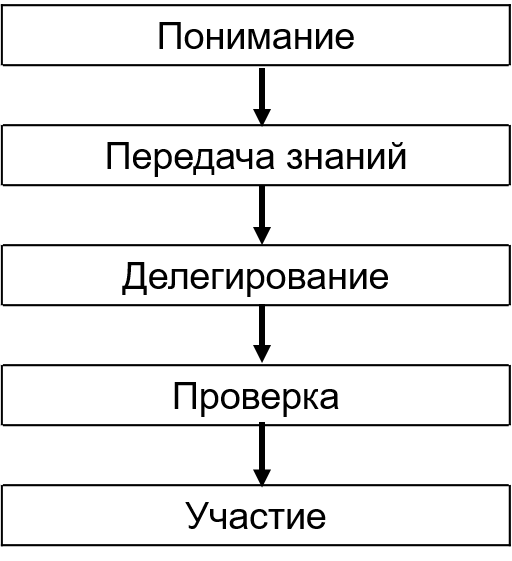
\includegraphics[width=129pt,height=190pt]{linear3.png}  
 \end{center}
\end{frame}


\begin{frame} \frametitle {Области деятельности}

Свое развитие основные принципы лидерства получают в~следующих областях деятельности:

\begin{itemize}
	\item Наставничество: учите окружающих учить
	\item Вознаграждение: награждая сотрудников за~выдающиеся результаты, вы сможете создать ситуацию, в которой одни успехи выливаются в другие
	\item Исправление:помогая сотрудникам учиться на~собственных ошибках, повышайте их~квалификацию
	\item Предвидение: предугадывайте проблемы, пока они не ударили по вашей команде
	\item Адаптация: совершенствуйтесь, извлекая уроки из~собственных ошибок
\end{itemize}
\end{frame}





\section{Сходства и различия между руководителем и лидером}

\begin{frame} \frametitle{Основные различия руководства и лидерства}

\begin{columns}
 		\column{0.5\textwidth}
 			\begin{block}{Руководитель}Руководство имеет место в~системе формальных (или официальных) отношений\end{block}
 		\column{0.5\textwidth}
 			\begin{block}{Лидер}Лидерство --- порождение системы неформальных отношений\end{block}
 	\end{columns}


\end{frame}



\begin{frame} \frametitle{Основные различия руководства и лидерства}

\begin{columns}
 		\column{4.8cm}
 			\begin{block}{Руководитель}Руководитель может не быть лидером, тогда эффективность его управления~снижается\hspace{28pt} \end{block}
 		\column{0.58\textwidth}
 			\begin{block}{Лидер}Лидер может быть руководителем (формальное лидерство), а может им и не являться, и иметь неформальную основу (неформальное лидерство)\end{block}
 	\end{columns}

\end{frame}



\begin{frame} \frametitle{Основные различия руководства и лидерства}

\begin{columns}
 		\column{0.56\textwidth}
 			\begin{block}{Руководитель}Руководитель \alert{определяет} какими способами нужно \alert{достигать} поставленные \alert{цели}, \alert{организует} и направляет \alert{работу членов команды} в соответствии с планами. Строит взаимодействие с окружающими на основе регламентации прав и~обязанностей, не выходит за их рамки, \alert{стремится к порядку и~дисциплине}\end{block}
 		\column{4.9cm}
 			\begin{block}{Лидер}Лидер реализует функции, ожидаемые коллективом и~\alert{самостоятельно} определяет его цели \vspace{95pt} \end{block}
 	\end{columns}

\end{frame}



\begin{frame} \frametitle{Основные различия руководства и лидерства}

\begin{columns}
 		\column{0.4\textwidth}
 			\begin{block}{Руководитель}Руководителю члены команды обязаны подчиняться, за что и~получают вознаграждение или~наказание
 			 \end{block}
 		\column{0.6\textwidth}
 			\begin{block}{Лидер}Лидер ведет за собой остальных, а~те выступают по отношению к~нему не подчиненными, а~последователями. Строит отношения с членами команды на~основе доверия\end{block}
 	\end{columns}

\end{frame}



\begin{frame} \frametitle{Основные сходства руководства и лидерства}

\begin{itemize}
	\item \alert{Руководитель} может быть \alert{лидером}, также как и \alert{лидер} может быть \alert{руководителем}
	\item И руководитель, и лидер имеют власть, хотя характер этой власти разный (личностный и организационный)
	\item И руководитель, и лидер влияют на окружающих, разница этих влияний в целях (личные цели или цели организации) и способах осуществления этого влияния
	
\end{itemize}

\end{frame}




\begin{frame} \frametitle {Лидерство руководителя}

\begin{block}{Вывод:}
Задача руководителя --- стать не формальным, а~подлинным лидером \end{block}
Это повышает неформальные организационные качества команды, эффективность и качество ее работы.\\
\vspace{5pt} \alert{Наиболее удачное сочетание:} одновременно руководитель и лидер
\end{frame}




\section{Командообразование (Teambuilding)}

\begin{frame} \frametitle{Понятие тимбилдинга}
\begin{block}{Определение:}
Тимбилдинг --- создание благоприятных условий для~работы команды, осуществление мероприятий, нацеленных на сплочение коллектива и~его организованности
\end{block}
\end{frame}

\lecturenotes Тимбилдинг (англ. Team building – построение команды). Этот термин получил распространение в бизнес среде как определение широкого диапазона действий для создания и повышения эффективности работы команды. Основа принципов тимбилдигна – это совместное времяпровождение. 
Первые игры, которые преследовали цель сплотить коллектив и выработать командный дух, появились в Великобритании в 40-х годах прошлого века. Они применялись для психологической и физической тренировки военнослужащих специальных подразделений Королевских военно-морских сил. 
Позднее метод перестал выполнять роль только корпоративного досуга, но и стал успешным способом объединения команды общей целью. В процессе выполнения конкретных заданий и костюмной игры, члены команды находили общие интересы и цели, что помогало сплотиться в трудовой деятельности. В РФ и странах содружества такое направление обозначилось в конце прошлого века.
Сначала это начало выражаться в бизнес-тренингах, но затем начали развиваться иные методы: творческие встречи, спортивные мероприятия, уроки психологии. Понятие тимбилдинг сегодня становится все шире, обрастая новыми способами объединения сотрудников, разрабатываются современные технологии.
Немало этому способствуют корпоративные вечеринки, на которых все активнее используются действия, нацеленные на сплочение коллектива.

\begin{frame} \frametitle{Задачи тимбилдинга}
\begin{itemize}
\item знакомство сотрудников разных отделов между собой
\item создание условий для неформального общения
\item повышение эффективности работы команды
\item повышение уровня взаимодействия между сотрудниками
\item сплочение коллектива

\end{itemize}
\end{frame}
\lecturenotes Независимо от размеров руководимой фирмы, числа ее сотрудников, для успешного ведения бизнеса необходимы сотрудники, составляющие единую команду, чтобы быть способными применять нестандартные ходы при выполнении обыденных работ. Тимбилдинг необходим:
- для всестороннего повышения мотивации сотрудников, создания крепких горизонтальных связей в фирме, открытия новых горизонтов в сфере командного духа, чтобы добиться лучшего взаимопонимания и доверия в коллективе;
- для повышения взаимодействия, сотрудничества, которое должно сменить чувства конкуренции;
- для воспитания чувства коллективизма и сплоченности.


\begin{frame} \frametitle{Задачи тимбилдинга}
\begin{itemize}

\item оценка роли каждого «игрока» в команде: выявление лидеров и аутсайдеров
\item освоение навыков решения нестандартных ситуаций
\item повышение мотивации на достижение коллективных целей
\item снятие стресса, усталости
\item возможность для сотрудников почувствовать себя в~новой роли
\end{itemize}
\end{frame}
\lecturenotes Тимбилдинг необходим для психологической разгрузки членов коллектива, на неформальном уровне повышения авторитета руководителя. Подобные мероприятия внедрить самостоятельно может далеко не каждый, чтобы достичь целей можно нанять специалистов – тренеров. Кроме этого, в настоящее время существуют специальные компании, предоставляющие подобные услуги, как тимбилдинг, которые могут заключаться как в тренинге, так и в играх на свежем воздухе.

\begin{frame} \frametitle{Виды тимбилдинга}
\begin{itemize}
\item Экстремальные
\item Интеллектуальные
\item Творческие
\end{itemize}
\end{frame}
\lecturenotes
Экстремальные. Связаны с экстремальными видами спорта и несут риск для здоровья или жизни. Данная группа мероприятий дает практически мгновенный результат и наиболее глубокое чувство единства

Интеллектуальные. Этнические, квесты, реалити шоу, ролевые мероприятия. Главный критерий – умственная работа и наличие смекалки. Отличный способ для участников проявить скрытые таланты и потенциал

Творческие. Решает такие вопросы, как построение отношений в коллективе на основании вкусовых предпочтений и глубокой эмоциональной сплоченности. В отличие от экстремальной группы, эффект достигается не так быстро, но, при регулярном проведении мероприятий – является более прочным и долговременным

\begin{frame} \frametitle{Примеры экстремального тимбилдинга}
\begin{itemize}
\item Приключенческие гонки
\item Ориентирование
\item Сплав на плотах
\end{itemize}
\end{frame}
\lecturenotes
Приключенческие гонки. Организуется тренинг формирования команды по принципу приключенческой гонки, проходящей в экстремальных условиях. Члены команды преодолевают дистанцию, выполняя различные задания и обязательно находя контрольные пункты. Участники не только преодолевают расстояние, но также проявляют свои знания, учась взаимодействовать и обсуждать планируемые действия

Ориентирование. Членам команды нужно с помощью компаса и карт находить необходимое количество пунктов, расположенных на местности. В рамках такого тимбилдинга каждый сотрудник может принимать решения, проявляя свои лидерские качества либо отрабатывая навыки подчиненного, необходимо соответствующее доверие и эффективные коммуникации в команде. Другим распространенным видом спорта становится джип-ориентирование – когда сотрудники на джипах ориентируются по заброшенной местности

Сплав на плотах. Сотрудники на мостах преодолевают водные препятствия, спускаясь по рекам. Здесь команде сотрудников предстоит самостоятельно добывать чистую воду, еду, защищать плот и преодолевать препятствия

\begin{frame} \frametitle{Примеры интеллектупльного тимбилдинга}
\begin{itemize}
\item Квест в городе/Ориентирование в городе
\item Старинные русские ремесла
\item Турнир по ролевым настольным играм
\item Турнир по шахматам
\end{itemize}
\end{frame}
\lecturenotes
Квест в городе / Ориентирование в городе. Организуется определенное состязание, головоломка с интенсивной коммуникацией внутри команды и проявлением творческих талантов

Старинные русские ремесла. Изучение старинных ремесел в виде чеканки, ковки, резьбы по дереву, гончарному ремеслу

\begin{frame} \frametitle{Примеры творческого тимбилдинга}
\begin{itemize}
\item Театральные постановки
\item Исторические тимбилдинги
\item Military
\item Литературные тимбилдинги
\item Кулинарные тимбилдинги
\end{itemize}
\end{frame}
\lecturenotes
Театральные постановки. Интересные театральные постановки являются основным звеном формирования команд, получая опыт коллективного взаимодействия. Работники самостоятельно организуют и ставят свой спектакль, а компания привлекает для этого профессионального режиссера

Исторические тимбилдинги. При составлении сценария мероприятия можно использовать различные исторические сюжеты и факты. Отличная возможность получить новые эмоции и яркий опыт. В том числе проведение рыцарских сражений, дней пионеров, походов викингов и пр.

Military. Военная атмосфера, артефакты, заброшенные полигоны – всё это позволит воссоздать идеальные условия для командного взаимодействия. Например, пейнтбол

Литературные тимбилдинги. Корпоратив с использованием литературных сюжетов, создавая отличные условия для командного творчества. Вечер чтения стихов собственного сочинения

Кулинарные тимбилдинги. Возможность проявить свои кулинарные таланты и познакомиться с интересными рецептами. Высокая степень эмоционального сплочения – с готовкой и поеданием интересных блюд. Команда учится взаимодействовать, проявляя свои таланты и лидерские качества в неформальной обстановке




\begin{thebibliography}{99}

%Информацию собирал с нескольких мест на один слайд, поэтому указал списком, а не метками

С. Архипенков Руководство командой разработчиков разработчиков ПО;
Государственный университет  - Высшая школа экономики Факультет Бизнес-информатики Учебное пособие «Лидерство и управление командой»;
Дж. Рейнвотер Как пасти котов 
https://www.kom-dir.ru/article/1127-razvitie-liderskih-kachestv
https://www.kom-dir.ru/article/1466-stili-liderstva
Ицхак Кальдерон Адизес Развитие лидеров. Как понять свой стиль управления и эффективно общаться с носителями иных стилей
\end{thebibliography}

\end{document}

%%% Local Variables: 
%%% mode: TeX-pdf
%%% TeX-master: t
%%% End: 
